\documentclass[a4paper, fleqn]{article}
\usepackage[utf8]{inputenc}
\usepackage{amsmath}
\usepackage{amssymb}
\usepackage{caption}
\usepackage{mathtools}
\usepackage{amsfonts}
\usepackage{lastpage}
\usepackage{tikz}
\usepackage{float}
\usepackage{textcomp}
\usetikzlibrary{patterns}
\usepackage{pdfpages}
\usepackage{gauss}
\usepackage{fancyvrb}
\usepackage[table]{colortbl}
\usepackage{fancyhdr}
\usepackage{graphicx}
\usepackage{pdfpages}
\usepackage{enumerate}
\usepackage[margin=2.5 cm]{geometry}

% algorithms
\usepackage{algorithm}      % algorithm float environment
\usepackage[noend]{algpseudocode}  % from algorithmicx; no "end" on functions
\newcommand*\Let[2]{\State #1 $\gets$ #2}
\newtheorem{theorem}{Theorem}
\algnewcommand{\LineComment}[1]{\State \(\sslash\) #1}
\algrenewcommand\algorithmiccomment[1]{\hfill\(\sslash\) #1}
\algrenewcommand\algorithmicrequire{\textbf{Precondition:}}

\setlength\parindent{0pt}
\setlength\mathindent{75pt}

\definecolor{listinggray}{gray}{0.9}
\usepackage{listings}
\lstset{
	language=,
	literate=
		{æ}{{\ae}}1
		{ø}{{\o}}1
		{å}{{\aa}}1
		{Æ}{{\AE}}1
		{Ø}{{\O}}1
		{Å}{{\AA}}1,
	backgroundcolor=\color{listinggray},
	tabsize=3,
	rulecolor=,
	basicstyle=\scriptsize,
	upquote=true,
	aboveskip={0.2\baselineskip},
	columns=fixed,
	showstringspaces=false,
	extendedchars=true,
	breaklines=true,
	prebreak =\raisebox{0ex}[0ex][0ex]{\ensuremath{\hookleftarrow}},
	frame=single,
	showtabs=false,
	showspaces=false,
	showlines=true,
	showstringspaces=false,
	identifierstyle=\ttfamily,
	keywordstyle=\color[rgb]{0,0,1},
	commentstyle=\color[rgb]{0.133,0.545,0.133},
	stringstyle=\color[rgb]{0.627,0.126,0.941},
  moredelim=**[is][\color{blue}]{@}{@},
}

\lstdefinestyle{base}{
  emptylines=1,
  breaklines=true,
  basicstyle=\ttfamily\color{black},
}

\pagestyle{fancy}
\def\checkmark{\tikz\fill[scale=0.4](0,.35) -- (.25,0) -- (1,.7) -- (.25,.15) -- cycle;}
\newcommand*\circled[1]{\tikz[baseline=(char.base)]{
            \node[shape=circle,draw,inner sep=2pt] (char) {#1};}}
\newcommand*\squared[1]{%
  \tikz[baseline=(R.base)]\node[draw,rectangle,inner sep=0.5pt](R) {#1};\!}
\newcommand{\comment}[1]{%
  \text{\phantom{(#1)}} \tag{#1}}
\def\el{[\![}
\def\er{]\!]}
\def\dpip{|\!|}
\def\MeanN{\frac{1}{N}\sum^N_{n=1}}
\cfoot{Page \thepage\ of \pageref{LastPage}}
\DeclareGraphicsExtensions{.pdf,.png,.jpg}
\author{Nikolaj Dybdahl Rathcke (Student ID: 74763954)}
\title{Cryptography and Coding Theory  \\ Assignment 3}
\lhead{Cryptography and Coding Theory}
\rhead{Assignment 3}

\begin{document}

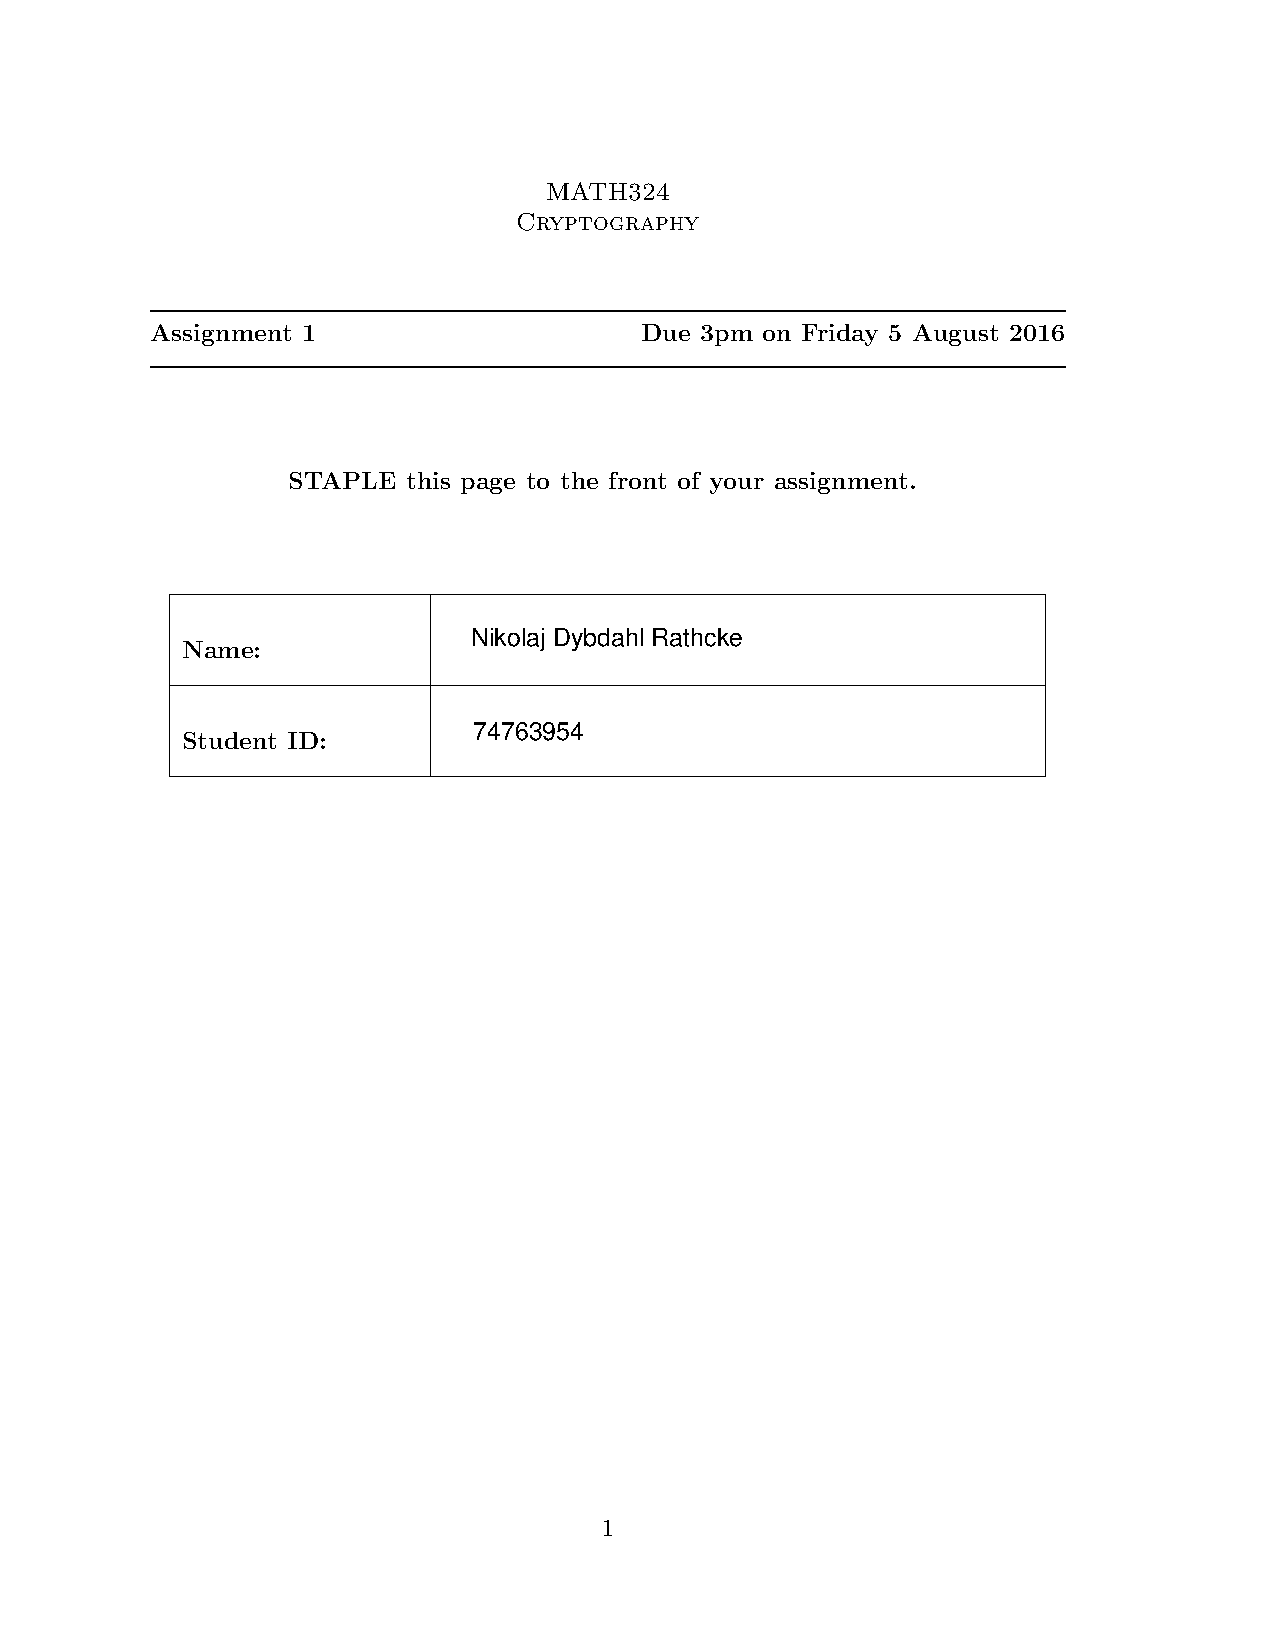
\includepdf[pages=1]{title.pdf}

\section{Question 1}
\subsection{(a)}
All $2^3$ codewords in $C$ is seen in Table \ref{tab1}.
\begin{table}[H]
  \centering
    \begin{tabular}{c|c}
      abc & xyz \\
      \hline
      000 & 000 \\
      \hline
      001 & 011 \\
      \hline
      010 & 101 \\
      \hline
      011 & 110 \\
      \hline
      100 & 110 \\
      \hline
      101 & 101 \\
      \hline
      110 & 011 \\
      \hline
      111 & 000
    \end{tabular}
    \caption{All codewords in $C$.}
    \label{tab1}
\end{table}
There are $4$ distinct binary string for $xyz$.

\subsection{(b)}
The minimum Hamming distance is $3$. To see this, note that every combination of $abc$
differs in at least one bit, which in turn means it will differ in two bits of $xyz$ (as
it is in two of equations). If two combinations differs in $2$ bits of $abc$, they will
differ in $2$ bits in $xyz$ as well (because two of equations for $xyz$ including \textit{one}
differing bit will change and the last one containing both will be the same). If they
differ in $3$ bits, $xyz$ will be the same, but it will still have a Hamming distance of
$3$.

\subsection{(c)}
Yes, the codewords is not in $C$ and does not satisfy the encoding, so an error must have
occurred. \\
We can determine the most likely codeword, since it has distance $1$ to $010101$, meaning
it cannot have distance $1$ to any other (otherwise, the minimum Hamming distance would
be $2$).

\subsection{(d)}
An error has occured. However, this time we cannot determine the most likely codeword as
it has minimum distance $2$ to another string. In this case it is easy to see that it
could be any of the three codewords that has $2$ zeroes in it.

\subsection{(e)}

\subsection{(f)}
Assuming the symbol error probability $p$ is the probability that a bit is flipped, the
probability the received word $s_2$ has a distance of no more than $1$ from the original
codewords $s_1$ (with length $6$) is:
\begin{align*}
  \mathbb{P}[\mbox{Codeword has $d(s_1, s_2)\leq 1$}] &=
  \mathbb{P}[d(s_1,s_2)=0]+\mathbb{P}[d(s_1,s_2)=1] \\
  &= (1-p)^6 + 6\left(p(1-p)^5\right) \\
  &= (1-p)^5(5p+1)
\end{align*}
which for larger $p$ quickly becomes very small.

\subsection{(g)}
If we take the second line in the calculation above, we get:
\begin{align*}
  (1-p)^6+6\left( p(1-p)^5\right) &=(1-p)^6+6p(1-p)^5
\end{align*}
To elaborate on the two terms. The first term is the case that each bit is not flipped.
It will not flip with probability $(1-p)$, so when we have $6$ bits, this does not happen
with probability $(1-p)^6$. \\
The second term is the case exactly one bit is flipped, i.e. that a bit is not flipped 5
times and flipped once. This yields $p(1-p)^5$. Since there $6$ combinations where one
bit is flipped, we multiply this by $6$.

\section{Question 2}
\subsection{(a)}
Using Theorem 1.6 from the lecture notes, we have that:
\begin{theorem}
  Let $C$ be a code.
  \begin{enumerate}[i]
    \item If $d(C)\geq s+1$, then $C$ can detect up to $t$ errors in any codeword. In
      other words, $C$ is a $s$-error correcting code.
    \item If $d(C)\geq 2t+1$, then $C$ can correct up to $t$ errors in any codeword. In
      other words, $C$ is a $t$-error correcting code.
    \item If $d(C)\geq 2t+s+1$, then $C$ can correct up to $t$ errors and simultaneously
      detect up to $s+t$ errors in any codeword.
  \end{enumerate}
\end{theorem}
In this case, $t=3$, so using $(ii)$, $C$ can correct a maximum of $3$ errors.

\subsection{(b)}
Using the same theorem as above, but this time using $(i)$, we get that $s=6$, so we can
detect a maximum of $6$ errors.

\subsection{(c)}
Yes we can. With $t=2$ and $s=2$, we satisfy the condition in $(iii)$ as $d(C)=7\geq
2t+s+1=7$. This means we can correct up to $t=2$ errors and detect $s+t=4$ errors.

\subsection{(d)}
No, we cannot. This implies $t=3$ and $s=1$ at minimum. This does not satisfy the
condition $(iii)$ as $2t+s+1=9\not \leq 7$.

\subsection{(e)}

\subsection{(f)}
For binary alphabet, the sphere-packing bounds is:
\begin{align*}
  M\sum_{i=0}^t \binom{n}{i}\leq 2^n
\end{align*}
If $d(C)=7$, we get that $t=\lfloor \frac{d-1}{2} \rfloor = 3$. We also know $C$ consists
of four words, so $M=4$. This gives us:
\begin{align*}
  M\sum_{i=0}^t \binom{n}{i}&= 4\sum_{i=0}^3 \binom{n}{i} \\
                            &= 4\left(1+n+\frac{n(n-1)}{2}+\frac{n!}{(n-3)!3!}\right) \\
                            &= \frac{2}{3}\left(n^3+5n+6\right)
\end{align*}
Solving for $n$ when setting this equal $2^n$ gives us the real solutions:
\begin{align*}
  x_1&\approx -0.956 \\
  x_2&\approx 11.045
\end{align*}
Obviously, $x_2$ is the solution we are looking for. This means we need $C$ to have at
least length $\lceil x_2\rceil=12$ or otherwise the bound is not satisfied.

\subsection{(g)}

\section{Question 3}
\subsection{(a)}
If we send a message through two channels, four different things can happen to a single
bit. Either it is transmitted correctly (flipped zero times), it is flipped in one of the
channels ($2$ of these cases) or it is flipped in both channels. If it is flipped either
zero times or twice, there is no error. Thus, the probability that it is flipped when the
message is received is just the sum of the two conditional probabilities that it is
flipped once, which we can define as $p_2$. \\
The probability that a bit is flipped once is:
\begin{align*}
  p_2 =\mathbb{P}[\mbox{Bit flipped once}] &=
  \mathbb{P}[\mbox{Flipped, not flipped}]+\mathbb{P}[\mbox{Not flipped, flipped}] \\
  &= p_1(1-p'_1)+(1-p_1)p'_1 \\
  &= p_1+p'_1-2p_1p'_1
\end{align*}

\subsection{(b)}

\subsection{(c)}
Every symbol error probability will tend to $1/2$ as $n$ goes to infinity, meaning the
received message of length $m$ will have an expected $m/2$ number of errors.

\subsection{(d)}
\subsubsection{(i)}
The number of times we can expect a symbol to change with $n$ channels and error
probability $p$ is:
\begin{align*}
\mathbb{E}[\mbox{\# of times flipped}] &= \sum_{i=1}^n p \\
                                         &= np \\
                                         &= 100\cdot 0.01 \\
                                         &= 1
\end{align*}
We can expect a bit to have been flipped once.

\subsubsection{(ii)}
It would be decoded to YES. If we calculate the probabilities that $000$ and $111$ turned
into $011$ with minimum number of flips, that is, we say $000$ did not flip its
first bit, but flipped the other bits only once, we get:
\begin{align*}
  \mathbb{P}[\mbox{YES originally}] &=(99/100)^{100}(100(1/100)(99/100)^{99})^2 &\approx
  0.05004 \\
  \mathbb{P}[\mbox{NO originally}]&=(100(1/100)(99/100)^{99})(99/100)^{100}(99/100)^{100}
  &\approx 0.04954
\end{align*}
Obviously, this is not conclusive proof. But, if we consider the rest of the cases (where
bits are flipped two or more times), these become more and more unlikely and I don't
think the probabilities for the rest of the cases (starting in $000$ and $111$) will
outweigh each other with more than $0.005$.

\section{Question 4}
\subsection{(a)}
We prove this with a constructive proof. \\
If we have two sequences $u$ and $v$ of length $n$ with $d(u,v)=a+b$, we know there are
$a+b$ places where they differ. Let the sequence $z$ be equal to both $u$ and $v$ in the
rest of the $n-a-b$ positions. Let $z$ be equal to $v$ in $a$ of the remaining $a+b$
positions and equal to $u$ in the other $b$ positions. \\
Since $z$ is a sequence that differs from $u$ only in the subsequence (not substring) of length $a$ where $u\neq z=b$, it must have $d(u,z)=a$. The same argument applies to $z$ and $v$ and so $d(v,z)=b$.

\subsection{(b)}
If we can correct up to $a$ errors, that means that for a received message with $a$
errors, we can uniquely determine the most likely codeword $s$. So $d(s,m)=a$. For any
other codeword $t$, we must have $d(t,m)\geq a+1$. \\
Note that any of the $a+1$ errors in $t$ are not in $s$ as otherwise $d(s,t)\geq 2a$ in
which case we can, from (a), construct another sequence $z$ that has distance $\leq a$ to
both $s$ and $t$. This would mean we could not uniquely determine a most likely codeword
to a message with $a$ errors as we have assumed. Putting this together, we get that
\begin{align*}
  d(s,t)&\geq a+(a+1) \\
        &= 2a+1
\end{align*}
Which is exactly what $(ii)$ in Theorem 1.6 says.

\end{document}
